% Provenance (never printed): see sources/outline_sources.md (Year 2: oceanic islands; growth,
% flank collapse and erosion of volcanic islands; reefs and atolls; subsidence). Hawaiian
% stages, slides, subsidence and drowned reefs after Clague and Sherrod (2014, USGS PP 1801
% ch. 3) and Denlinger and Morgan (2014, ch. 4); the Nuuanu slide after the ODP Leg 200 report;
% the Enewetak holes after Ladd and Schlanger (1960, USGS PP 260-Y); Kure after the NOAA
% monument pages; the depth--age law from the Book 2 and Book 3 rows. Curves and the invented
% Petrel island from figdata/bachelor-2/islands.py; exercise and problem values in the Book 4
% scratch calculator calc/ch17.py.
\chapter{Oceanic Islands}\label{ch:b2:oceanic-islands}

In 1952, on two islands of Enewetak \omterm{def:b2:oceanic-islands:reefs}{Atoll} in the western Pacific (then spelled Eniwetok), two
drill holes went down through coral rock to more than \qty{1.2}{km}. On Parry Island, the bit
brought up cuttings of fresh basalt at a depth of 4,158 feet, \qty{1267}{m}, and then a core of
olivine basalt. Above it lay limestone of Eocene age, full of reef corals of a kind that does not
grow deeper than about \qty{46}{m}. A coral reef had once grown on the shoulders of a volcano near
sea level, and the volcano had sunk by more than a kilometre while the reef kept growing on top of
it. This chapter follows an \omterm{def:b2:oceanic-islands:stages}{oceanic island} through its whole life: how it grows, how its flanks
fall into the sea, why it sinks, and how a ring of coral can outlive it.
% ledger: ls60:enewetak, ics4:eocene

\begin{recall}
\textbf{From the Year 1 volume}: hotspot, mantle plume, hotspot track and its age progression,
the Hawaiian--Emperor chain and the Hawaiian swell; the depth--age law of the ocean floor; reefs,
their fringing, barrier and \omterm{def:b2:oceanic-islands:reefs}{atoll} forms as Darwin described them, and the rule ``keep up or
drown''; eustasy and the sea level of the last glacial maximum, about \qty{120}{m} lower than
today. \textbf{From the school volumes}: the shield volcano; the wave-cut platform.
\textbf{From \cref{ch:b2:magmatic-series}}: tholeiitic and \omterm{def:b2:magmatic-series:series}{alkaline series}.
\end{recall}

\section{The growth of a volcanic island}\label{sec:b2:oceanic-islands:growth}

The Hawaiian Islands are the youngest end of the chain that the Year 1 volume followed across the
northern Pacific. The main islands hold 19 known shield volcanoes: 15 stand above the sea,
3 are submerged, and one, newly born, is still under water. As the Pacific plate carries them
north-west, each is born above the hotspot, grows, dies as it drifts away, and sinks. The life is
regular enough to be cut into stages.
% ledger: cs14:volcanoes

\begin{definition}[Oceanic island; stages of growth]\label{def:b2:oceanic-islands:stages}
An \emph{oceanic island}\index{oceanic island} is a volcanic island that rises from the ocean
floor, built on oceanic lithosphere. An island of a hotspot chain passes through four eruptive
stages: a \emph{preshield} stage of small eruptions of alkalic lava on the sea floor; the
\emph{shield stage}\index{shield stage}, in which tholeiitic lava builds the bulk of the volcano
while it lies over the hotspot; a \emph{postshield} stage of fewer, more alkalic eruptions,
which cap the shield; and, after a pause, a \emph{rejuvenated} stage of rare, small alkalic
eruptions. Erosion and sinking then take over.
\end{definition}
% ledger: usgs14:hawaii-stages, cs14:rejuvenated

The stages follow the supply of heat. Loihi, the newest volcano, lies \qty{54}{km} south of the
summit of Kilauea; its top is still \qty{975}{m} under the sea but already \qty{2.5}{km} above the
sea floor around it, and its oldest lavas are alkalic. In the \omterm{def:b2:oceanic-islands:stages}{shield stage}, the volcano lies over
the hotspot and is fed at the highest rate. Each Hawaiian volcano erupts an estimated 80 to
\qty{95}{\percent} of its final volume in this stage, mostly within its first 1 to \qty{2}{Myr}.
Late in the stage the rate of eruption drops by a factor of ten. The shallow \omterm{def:b2:magma-emplacement:magma}{magma} reservoirs, 1
to \qty{7}{km} deep, can no longer be kept alive, though smaller ones at 20 to \qty{30}{km}
remain. The lava turns alkalic again, because a lower degree of melting gives it, as
\cref{ch:b2:magmatic-series} showed. The rejuvenated stage comes after a pause of 2.0 to less
than \qty{0.5}{Myr}. It can be one or two episodes, or very long: on Niihau it lasted from 2.2 to
\qty{0.4}{Ma}, and on Kauai it has gone on since \qty{3.5}{Ma}.
% ledger: cs14:loihi, usgs14:hawaii-stages, cs14:rejuvenated

The volumes are enormous. The volume of Mauna Loa is estimated at about \qty{74000}{km^3}. When the boundary with Kilauea is drawn again so that Kilauea keeps only about
\qty{10000}{km^3}, Mauna Loa's share rises to \qty{95600}{km^3}. Young Loihi holds
\qty{1700}{km^3}. The whole chain, since \qty{81}{Ma}, comes to about
\qty{2e6}{km^3}, an average of \qty{0.07}{km^3} a year. The load is heavy enough to bend the
plate: the oceanic crust under the islands is pressed down by as much as \qty{5}{km}, along a
trough called the Hawaiian Moat, and a low bulge, the Hawaiian Arch, rises a few hundred
kilometres away. How a plate bends under a load is taken up in the Year~3 volume. Here the moat
matters because it is where much of the debris of the islands ends up.
% ledger: cs14:volumes, cs14:loihi, cs14:moat

\begin{omfigure}
\centering
\begin{tikzpicture}[x=0.95cm, y=0.95cm, font=\footnotesize]
% schematic, not to scale (vertical exaggeration about 10). Sea level y = 0; sea floor
% y = -1.6 - 0.0625 (16 - x), deepening with the age of the plate to the left.
\fill[omSea!45] (0,0) -- (16,0) -- (16,-1.6) -- (0,-2.6) -- cycle;
\fill[black!18] (0,-2.6) -- (16,-1.6) -- (16,-3.1) -- (0,-3.1) -- cycle;
\draw[black!60] (0,-2.6) -- (16,-1.6);
\draw[omSea!60!black] (0,0) -- (16,0);
\node[anchor=south, font=\scriptsize] at (8.7,0) {sea level};
% (a) shield stage over the hotspot
\fill[lith basalt, draw=black!70] (12.6,-1.8125) -- (13.9,0.75) -- (14.3,0.9) -- (14.7,0.75) -- (16,-1.6) -- cycle;
% (b) eroded island with a fringing reef (valleys notched in the summit)
\fill[lith basalt, draw=black!70] (9.2,-2.025) -- (10.1,0.15) -- (10.3,0.35) -- (10.45,0.2) -- (10.6,0.45) -- (10.8,0.25) -- (11.0,0.3) -- (11.2,0.1) -- (12.0,-1.85) -- cycle;
\fill[lith reef limestone, draw=black!70] (10.038,0) -- (9.976,-0.15) -- (9.80,0) -- cycle;
\fill[lith reef limestone, draw=black!70] (11.241,0) -- (11.303,-0.15) -- (11.46,0) -- cycle;
% (c) barrier reef around a smaller island, a lagoon between
\fill[lith basalt, draw=black!70] (5.8,-2.2375) -- (7.0,0.2) -- (8.2,-2.0875) -- cycle;
\fill[lith reef limestone, draw=black!70] (6.384,-1.05) -- (6.42,0) -- (6.60,0) -- (6.62,-0.45) -- (6.680,-0.45) -- cycle;
\fill[lith reef limestone, draw=black!70] (7.656,-1.05) -- (7.62,0) -- (7.44,0) -- (7.42,-0.45) -- (7.341,-0.45) -- cycle;
% (d) atoll: volcano bevelled and drowned, reef cap with a lagoon
\fill[lith basalt, draw=black!70] (2.7,-2.43125) -- (3.6,-0.55) -- (4.0,-0.55) -- (4.9,-2.29375) -- cycle;
\fill[lith reef limestone, draw=black!70] (3.4325,-0.9) -- (3.47,0) -- (4.14,0) -- (4.1806,-0.9) -- (4.0,-0.55) -- (3.6,-0.55) -- cycle;
\fill[omSea!45] (3.62,-0.15) rectangle (3.99,0);
% (e) guyot: flat top with a drowned reef cap, beyond the Darwin point
\fill[lith basalt, draw=black!70] (0.2,-2.5875) -- (0.9,-0.95) -- (1.7,-0.95) -- (2.4,-2.475) -- cycle;
\fill[lith reef limestone, draw=black!70] (0.9,-0.95) -- (0.96,-0.75) -- (1.64,-0.75) -- (1.7,-0.95) -- cycle;
% Darwin point
\draw[black!70, dashed] (2.55,0.55) -- (2.55,-2.5);
\node[anchor=south, font=\scriptsize] at (2.55,0.55) {Darwin point};
% hotspot and plate motion
\draw[omThm, line width=1.4pt, -{Stealth[length=2.5mm]}] (14.3,-3.9) -- (14.3,-3.15);
\node[anchor=west, font=\scriptsize, text=omThm] at (14.4,-3.7) {hotspot};
\draw[black, line width=0.8pt, -{Stealth[length=2.5mm]}] (9.5,-2.85) -- (6.5,-2.85);
\node[anchor=west, font=\scriptsize] at (9.6,-2.85) {plate motion};
\node[anchor=west, font=\scriptsize] at (0.1,-2.9) {oceanic lithosphere};
% stage labels
\node[align=center, font=\scriptsize] at (14.3,1.45) {(a) shield stage};
\node[align=center, font=\scriptsize] at (10.6,1.3) {(b) eroded island,\\ fringing reef};
\node[align=center, font=\scriptsize] at (7.0,1.45) {(c) barrier reef};
\node[align=center, font=\scriptsize] at (3.8,1.45) {(d) atoll};
\node[align=center, font=\scriptsize] at (1.3,1.45) {(e) guyot};
\draw[black!60, -{Stealth[length=2mm]}] (13.6,-3.7) -- (0,-3.7);
\node[anchor=south, font=\scriptsize, fill=white, inner sep=1pt] at (7,-3.7) {older volcanoes, older and deeper plate};
\end{tikzpicture}
\par\smallskip{\small The life of an \omterm{def:b2:oceanic-islands:stages}{oceanic island}, read along a hotspot chain (schematic, not to
scale, vertical scale much exaggerated). The plate carries each volcano away from the hotspot
(right) and the volcano sinks with it, while erosion wears it down. (a)~A shield volcano grows over
the hotspot. (b)~Extinct and eroded, it is fringed by reefs. (c)~Sunk further, it is surrounded
by a \omterm{def:b2:oceanic-islands:reefs}{barrier reef} with a lagoon behind. (d)~Its summit is gone below the sea, and a reef cap with
a central lagoon, an \omterm{def:b2:oceanic-islands:reefs}{atoll}, grows on top of it. (e)~Carried into water too cool for the reef to
keep up, the \omterm{def:b2:oceanic-islands:reefs}{atoll} drowns and sinks as a flat-topped \omterm{def:b2:oceanic-islands:seamount}{guyot}.}
\end{omfigure}
% ledger: cs14:volcanoes, cs14:erase, cs14:darwin-point, pmnm:geology

\section{Flank collapse}\label{sec:b2:oceanic-islands:collapse}

A volcano several kilometres high, built of loose lava flows and rubble, standing on slopes that
go down into the moat, is not stable. In 1975 the Kalapana earthquake, of magnitude 7.7, moved
the south flank of Kilauea up to \qty{10}{m} towards the sea in one go and raised a tsunami. In
1868, another flank movement came with a magnitude 7.9 earthquake and a tsunami that killed 46
people. Seismic profiles under these flanks show a deep reflector. It is read as a
\omterm{def:b2:alpine-orogen:decollement}{décollement} along the top of the old oceanic crust, on which the whole flank slides. Usually the
flank creeps; sometimes it fails.
% ledger: dm14:flank

\begin{definition}[Flank collapse; debris avalanche; slump]\label{def:b2:oceanic-islands:collapse}
A \emph{flank collapse}\index{flank collapse} is the failure of a large part of the flank of a
volcano, which slides away under its own weight. When the moving mass breaks up and runs out
fast, as a flow of blocks and rubble that can travel far beyond the foot of the volcano, it is a
\emph{debris avalanche}\index{debris avalanche}. When it moves slowly, as large blocks rotating
on faults rooted in a deep \omterm{def:b2:alpine-orogen:decollement}{décollement} and staying near the volcano, it is a \emph{slump}.
\end{definition}

The evidence lies under the sea. In the late 1980s, sidescan sonar mapping of the waters around
the Hawaiian Islands showed debris strewn over the deep sea floor, several hundred kilometres from
the islands, and slumps made of large segmented blocks. Seventeen large slides were identified
around the main islands, formed in the past \qty{5}{Myr}. Seventy are now known along the
Hawaiian Ridge between the Island of Hawaii and Midway, formed over \qty{30}{Myr}. That is at
least one slide every \qty{300}{kyr} around the main islands. These counts are minima, since a
younger volcano can bury the scar and the debris of an older one: the summit \omterm{def:b2:eruptive-styles:caldera}{caldera} and a rift zone
of Niihau are missing, and no deposit has been found for them. The giant slides seem most likely while the
volcano grows fastest, from the late preshield to the early postshield stage, but they continue
long after.
% ledger: cs14:slides, dm14:flank

The largest is the Nuuanu landslide, which tore off the north-eastern flank of the Koolau
volcano on Oahu. It is a \omterm{def:b2:oceanic-islands:collapse}{debris avalanche} spread over \qty{23000}{km^2}, extending more than
\qty{200}{km} from the island. Its blocks include Tuscaloosa \omterm{def:b2:oceanic-islands:seamount}{Seamount}, about \qty{30}{km} long,
\qty{17}{km} wide and at least \qty{2}{km} tall. The avalanche crossed the deep moat and climbed
more than \qty{100}{km} up the slope of the Hawaiian Arch. Its age is estimated at 2.1 to
\qty{1.8}{Ma}, near the end of the life of Koolau or after it, whose surface lavas are 1.8 to
\qty{2.6}{Ma} old. How many collapses it was made of, and how thick it is far from the island,
are still open questions.
% ledger: odp200:nuuanu

\begin{omfigure}
\centering
\begin{tikzpicture}[x=0.95cm, y=0.95cm, font=\footnotesize]
% schematic section from the summit of an island (left) across the moat to the arch (right);
% not to scale. Sea level y = 0; top of the old oceanic crust, bent down under the island.
\fill[omSea!45] (0,0) -- (15,0) -- (15,-2.2) -- (13.5,-2.12) -- (11,-2.05) -- (8.5,-2.35) -- (6.5,-2.75) -- (5.6,-2.82) -- (4.0,-1.4) -- (2.5,0) -- cycle;
\fill[black!18] (0,-3.05) -- (5.6,-2.82) -- (6.5,-2.75) -- (8.5,-2.35) -- (11,-2.05) -- (13.5,-2.12) -- (15,-2.2) -- (15,-3.6) -- (0,-3.6) -- cycle;
\draw[black!70] (0,-3.05) -- (5.6,-2.82) -- (6.5,-2.75) -- (8.5,-2.35) -- (11,-2.05) -- (13.5,-2.12) -- (15,-2.2);
\draw[omSea!60!black] (0,0) -- (15,0);
\node[anchor=south east, font=\scriptsize] at (15,0) {sea level};
% the volcano: present flank (after collapse) and the lost flank (dashed)
\fill[lith basalt, draw=black!70] (0,1.15) -- (0.8,1.05) -- (1.25,0.95) -- (1.45,0.45) -- (1.75,0.1) -- (2.6,-0.75) -- (3.6,-1.6) -- (4.6,-2.4) -- (5.6,-2.82) -- (0,-3.05) -- cycle;
\draw[black!70, dashed] (1.25,0.95) -- (2.5,0) -- (4.0,-1.4) -- (5.6,-2.82);
\node[font=\scriptsize, align=center, fill=white, inner sep=1pt] at (0.8,-1.6) {volcano};
\node[font=\scriptsize, anchor=south west, align=left] at (2.0,0.25) {scar of the\\ lost flank};
% slump: blocks rotated on listric faults rooted in the decollement
\draw[black, line width=0.7pt] (1.45,0.45) .. controls (1.7,-1.4) and (2.4,-2.6) .. (3.6,-2.95);
\draw[black, line width=0.7pt] (2.6,-0.75) .. controls (2.8,-1.8) and (3.3,-2.6) .. (4.4,-2.9);
\draw[omThm, line width=1.1pt] (0.6,-3.03) -- (5.6,-2.82);
\node[anchor=north, font=\scriptsize, text=omThm] at (2.9,-3.05) {décollement};
% debris avalanche: hummocky sheet across the moat and up the arch, with blocks
\fill[lith conglomerate, draw=black!70] (4.6,-2.4) -- (5.6,-2.62) -- (6.5,-2.6) -- (8.5,-2.22) -- (11,-1.95) -- (12.6,-2.03) -- (11,-2.05) -- (8.5,-2.35) -- (6.5,-2.75) -- (5.6,-2.82) -- cycle;
\fill[lith basalt, draw=black!70] (7.0,-2.62) -- (7.25,-2.25) -- (7.95,-2.22) -- (8.1,-2.43) -- cycle;
\fill[lith basalt, draw=black!70] (9.3,-2.2) -- (9.45,-2.02) -- (9.75,-2.0) -- (9.85,-2.17) -- cycle;
\fill[lith basalt, draw=black!70] (10.6,-2.05) -- (10.7,-1.93) -- (10.9,-1.92) -- (10.95,-2.03) -- cycle;
\draw[black!70] (7.6,-2.2) -- (7.4,-1.3) node[anchor=south, font=\scriptsize, align=center] {block several\\ km across};
\node[anchor=south, font=\scriptsize, align=center] at (10.3,-1.3) {debris avalanche};
\draw[black!70] (10.3,-1.3) -- (10.0,-1.98);
\node[font=\scriptsize] at (6.6,-3.2) {moat};
\node[font=\scriptsize] at (11.6,-2.6) {arch};
\node[anchor=west, font=\scriptsize] at (12.6,-3.3) {oceanic crust};
\draw[black!70] (2.55,-1.55) -- (3.35,-0.6) node[anchor=west, font=\scriptsize, inner sep=1pt] {slump};
\draw[black!60, {Stealth[length=2mm]}-{Stealth[length=2mm]}] (5.6,-3.95) -- (12.6,-3.95);
\node[anchor=north, font=\scriptsize] at (9.1,-3.95) {up to about \qty{200}{km}};
\end{tikzpicture}
\par\smallskip{\small \omterm{def:b2:oceanic-islands:collapse}{Flank collapse} of an \omterm{def:b2:oceanic-islands:stages}{oceanic island} (schematic, not to scale). Near the
volcano, a slump moves slowly as rotating blocks on faults that root in a \omterm{def:b2:alpine-orogen:decollement}{décollement} at the top
of the old oceanic crust. A \omterm{def:b2:oceanic-islands:collapse}{debris avalanche} breaks off the flank, leaving a scar, and runs out as
a sheet of rubble carrying blocks several kilometres across. The Nuuanu avalanche crossed the moat
and climbed onto the arch, more than \qty{200}{km} from Oahu.}
\end{omfigure}
% ledger: dm14:flank, odp200:nuuanu, cs14:moat

A slide that falls into the sea pushes the water aside. On Lanai and Molokai, chaotic breccias
of coral and lava stand up to \qty{155}{m} above sea level and have been read as the deposits of
giant waves raised by collapses. The reading is disputed. Some authors explain the deposits by an
uplift of the islands, though drowned reefs south of Lanai show no sign of such an uplift.
Roughly a third of the giant Hawaiian slides were \omterm{def:b2:oceanic-islands:collapse}{debris avalanches} able to raise huge waves. How
such a hazard is weighed, rare but very large, is a question for \cref{ch:b2:geological-hazards}.
% ledger: cs14:megatsunami

\section{Why oceanic islands sink}\label{sec:b2:oceanic-islands:subsidence}

Two processes make an \omterm{def:b2:oceanic-islands:stages}{oceanic island} sink, and they overlap. The first is loading: as the volcano
grows, its weight pushes the plate down. This rapid phase lasts perhaps a million years and
drowns shorelines and reefs by more than a kilometre. Off the north-west coast of the Island of
Hawaii, dated drowned reefs give a sinking rate of \qty{2.6}{m} per thousand years. A small
volcano can drown entirely in this phase: Mahukona, beside the Island of Hawaii, was briefly an
island and now has its summit at about \qty{1100}{m} under water. The second process is the
cooling of the plate, which goes on for a hundred million years, and which this section puts in
numbers.
% ledger: cs14:subsidence, cs14:mahukona

The Year 1 volume measured how the ocean floor deepens with its age $t$ (in \unit{Myr}). In the
form used in this chapter:
\[
d(t) = \qty{2500}{m} + C\sqrt{t}, \qquad C = \qty{350}{m.Myr^{-1/2}}, \qquad 0 \le t \le 70,
\]
and, for plates older than about \qty{20}{Myr},
\[
d(t) = \qty{6400}{m} - \qty{3200}{m}\; e^{-t/62.8}.
\]
The two forms agree within about \qty{20}{m} between 20 and \qty{50}{Myr}, and cross at
\qty{26}{Myr}.
% ledger: ps77:depth-age (Book 2), parsons:plate-model (Book 3)
% values (islands.py): t_switch 26.27, d_switch 4293.8; root - exp: 20 Myr -7.6, 50 Myr +18.3

\begin{proposition}[Thermal sinking of an island]\label{prop:b2:oceanic-islands:sinking}
An island built on a plate of age $t_1$, carried with the plate, loading it with a weight that
no longer changes and leaving the cooling of the plate under it unchanged, sinks by
\[
S = d(t_2) - d(t_1)
\]
by the time the plate has reached the age $t_2$, at the rate $\dot S = d'(t)$. With the root law,
\[
S = C\left(\sqrt{t_2} - \sqrt{t_1}\right), \qquad \dot S = \frac{C}{2\sqrt t},
\]
and, with the exponential law, $\dot S = (\qty{3200}{m}/\qty{62.8}{Myr})\,e^{-t/62.8}$. Over a
given interval, a young plate carries its islands down further than an old one.
\end{proposition}

\begin{proof}
Compare two columns of the plate, of the same age, one under the island and one under the open
ocean far away. Both cool the same way, since the island leaves the cooling of the plate unchanged. So both contract by the same amount, and the top of each goes down by the same
amount. The island's own weight is already balanced and no longer changes, so it adds nothing
more. The open-ocean column goes down by $d(t_2) - d(t_1)$; so does the island. Differentiating
gives the rate. For the last claim: over a fixed interval $\Delta$, $C(\sqrt{t_1 + \Delta} -
\sqrt{t_1})$ decreases as $t_1$ grows, since its derivative, $\frac C2\bigl(1/\sqrt{t_1 + \Delta}
- 1/\sqrt{t_1}\bigr)$, is negative.
\end{proof}

The proposition leaves out two things on purpose. The swell of the hotspot lifts the plate as it
passes and lets it down again as it moves away, which adds to the sinking of the youngest islands
(the Year 1 volume measured the swell). And a load changes while the volcano grows, which is the
rapid phase above. Once both are over, the island follows the floor.

The rates are small. On a plate \qty{4}{Myr} old, the root law gives \qty{87.5}{m} per million
years, less than a tenth of a millimetre a year. On a plate \qty{100}{Myr} old, the exponential
law gives \qty{10.4}{m} per million years, or \qty{0.01}{m} per thousand years. That is the rate
measured along much of the Hawaiian Ridge and the Emperor \omterm{def:b2:oceanic-islands:seamount}{Seamounts}. The loading phase, at
\qty{2.6}{m} per thousand years, is some 250 times faster.
% ledger: cs14:subsidence; values (islands.py): rate_100 10.37, age_rate10 102.3

\begin{omfigure}
\centering
% figdata/bachelor-2/islands.py part sink
\begin{tikzpicture}
\begin{axis}[width=0.8\linewidth, height=6.2cm, y dir=reverse, xmin=0, xmax=100, ymin=0,
  ymax=3000, xlabel={time since the island was built (\unit{Myr})},
  ylabel={thermal sinking (\unit{m})}, tick label style={font=\scriptsize},
  label style={font=\small}, xtick pos=bottom, ytick pos=left]
\addplot[omThm, line width=1pt] table[x=dt_Myr, y=t2] {figdata/out/bachelor-2-islands-sink.dat};
\addplot[orange!80!black, line width=1pt] table[x=dt_Myr, y=t10] {figdata/out/bachelor-2-islands-sink.dat};
\addplot[blue!70!black, line width=1pt] table[x=dt_Myr, y=t30] {figdata/out/bachelor-2-islands-sink.dat};
\addplot[black!45, line width=1pt] table[x=dt_Myr, y=t60] {figdata/out/bachelor-2-islands-sink.dat};
\node[font=\scriptsize, anchor=south east, inner sep=1pt] at (axis cs:99,2470) {plate \qty{2}{Myr} old};
\node[font=\scriptsize, anchor=south east, inner sep=1pt] at (axis cs:99,2140) {\qty{10}{Myr}};
\node[font=\scriptsize, anchor=south east, inner sep=1pt] at (axis cs:99,1380) {\qty{30}{Myr}};
\node[font=\scriptsize, anchor=south east, inner sep=1pt] at (axis cs:99,710) {\qty{60}{Myr}};
\draw[black!50, dashed] (axis cs:0,1267) -- (axis cs:58,1267);
\node[font=\scriptsize, anchor=north west, inner sep=1pt] at (axis cs:1,1300) {Enewetak, \qty{1267}{m}};
\end{axis}
\end{tikzpicture}
\par\smallskip{\small Thermal sinking of an island carried by its plate, from the depth--age law,
for islands built on plates 2, 10, 30 and \qty{60}{Myr} old (the root law up to a plate age of
\qty{26}{Myr}, the exponential law beyond, where the two meet). The younger the plate, the faster
and further the island sinks. The dashed line marks the depth of the basalt under Enewetak, the
thickness of reef rock that sinking has to make room for.}
\end{omfigure}
% ledger: ps77:depth-age (Book 2), parsons:plate-model (Book 3), ls60:enewetak

\section{Reefs, atolls and guyots}\label{sec:b2:oceanic-islands:reefs}

The Year 1 volume described the three forms of reef as Darwin explained them, from a reef fringing
an island to a ring of coral around a lagoon, and ended on a question: why do the islands sink,
and how far? The previous section answered it. The forms can now be defined by the state of the
island underneath.

\begin{definition}[Fringing reef; barrier reef; atoll]\label{def:b2:oceanic-islands:reefs}
A \emph{fringing reef}\index{fringing reef} is a reef attached to the shore of an island, with no
lagoon, or only a narrow, shallow channel, between them. A \emph{barrier reef}\index{barrier reef}
is a reef separated from the shore by a lagoon, on the flanks of an island that has sunk while the
reef grew upward. An \emph{atoll}\index{atoll} is a ring of reef, with low islands of reef debris,
around a lagoon with no volcanic rock above sea level: its volcano lies entirely under the reef.
\end{definition}

\begin{definition}[Seamount; guyot]\label{def:b2:oceanic-islands:seamount}
A \emph{seamount}\index{seamount} is a volcano on the ocean floor whose summit lies below sea
level, either because it never reached the surface or because it has sunk. A
\emph{guyot}\index{guyot} is a seamount with a flat top, cut by waves or capped by a reef when
it stood at sea level, and then drowned.
\end{definition}

If a reef keeps its top at sea level while the volcano sinks under it, the reef rock piles up as
fast as the island goes down. The thickness of the cap then records the sinking.

\begin{proposition}[Thickness of a reef cap]\label{prop:b2:oceanic-islands:cap}
Let the last volcanic rock of an island go below sea level when its plate is $t_1$ old, and let a
reef keep its top at sea level from then on, until the plate is $t_2$ old. If sea level has risen
by $\Delta\eta$ between the two times (relative to the centre of the Earth), then the reef cap
over the volcano is
\[
H = d(t_2) - d(t_1) + \Delta\eta = C\left(\sqrt{t_2} - \sqrt{t_1}\right) + \Delta\eta
\]
thick, the second form with the root law. It does not depend on the rate at which the reef can
grow, provided that rate is never smaller than the relative rise of sea level.
\end{proposition}

\begin{proof}
At $t_1$ the top of the volcano is at sea level; at $t_2$ it lies $S = d(t_2) - d(t_1)$ lower by
\cref{prop:b2:oceanic-islands:sinking}, while the sea surface has risen by $\Delta\eta$. The top
of the reef is at the sea surface at both times, and its base is the top of the volcano. So the
thickness is the distance between them, $S + \Delta\eta$. A reef that keeps up stops at the
surface, so a faster reef does not build a thicker cap; a reef that cannot keep up falls behind
and drowns, which is the rule recalled from the Year 1 volume.
\end{proof}

Enewetak bears this out. On the root law, a cap of \qty{1267}{m} needs $\sqrt{t_2} - \sqrt{t_1} =
1267/350 = 3.62$: for example, a volcano bevelled to sea level on a plate \qty{10}{Myr} old and
carried until the plate is \qty{46}{Myr} old. That is \qty{36}{Myr}, the order of time that
separates the Eocene base of the limestone from today. The drill holes also showed what the
proposition leaves out. Leached zones, where the aragonite of the corals has been dissolved or
recrystallised, record times when the top of the \omterm{def:b2:oceanic-islands:reefs}{atoll} stood above the sea and rain fell on it.
Sea level falls and rises with the ice ages, and the cap has been exposed and drowned again many
times on its way down.
% ledger: ls60:enewetak, ics4:eocene; calc/ch17.py: (3.162 + 3.620)^2 = 46.0

\begin{history}[Drilling through atolls, 1896--1952]
Darwin's theory made a prediction that could be checked only with a drill: under an \omterm{def:b2:oceanic-islands:reefs}{atoll} there
should be a thick pile of shallow-water reef rock, resting on volcanic rock. The first deep hole
on a Pacific \omterm{def:b2:oceanic-islands:reefs}{atoll} was drilled at Funafuti from 1896 to 1898 and stopped at 1,114 feet,
\qty{340}{m}, without reaching the volcano. A hole on Kita-daito-jima, south of Japan and east of Okinawa,
reached 1,416 feet in 1936, and one on Bikini 2,556 feet in 1947, neither of them reaching it. The holes on Enewetak, in
1951 and 1952, were the first to reach the foundation of an \omterm{def:b2:oceanic-islands:reefs}{atoll}. On Elugelab, hard basement was
struck at 4,610 feet; on Parry Island, basalt at 4,158 feet, 450 feet higher, \qty{22}{miles}
away. The drillers had found a basaltic volcano that rises two miles above the ocean floor, capped
by reef limestone since the Eocene. Elugelab was destroyed in a test of a thermonuclear device
shortly after the drilling ended.
\end{history}
% ledger: ls60:holes, ls60:enewetak

\begin{omfigure}
\centering
% figdata/bachelor-2/islands.py part holes
\begin{tikzpicture}
\begin{axis}[width=0.8\linewidth, height=6.0cm, ybar, bar width=16pt, y dir=reverse, ymin=0,
  ymax=1500, enlarge x limits=0.1, symbolic x coords={Funafuti,Kita-daito-jima,Bikini,Eniwetok-K-1B,Eniwetok-F-1,Eniwetok-E-1},
  xtick=data, xticklabels={{Funafuti\\1898},{Kita-daito-jima\\1936},{Bikini\\1947},{Enewetak\\K-1B, 1951},{Enewetak\\F-1, 1952},{Enewetak\\E-1, 1952}},
  xticklabel style={align=center, font=\scriptsize}, ylabel={depth (\unit{m})},
  tick label style={font=\scriptsize}, label style={font=\small}, xtick pos=bottom, ytick pos=left]
\addplot[fill=omLithLime, draw=black!70] table[x=name, y=td_m] {figdata/out/bachelor-2-islands-holes.dat};
\addplot[only marks, mark=-, mark size=9pt, line width=2.2pt, black, unbounded coords=discard, xshift=0pt]
  table[x=name, y=basalt_m] {figdata/out/bachelor-2-islands-holes.dat};
\end{axis}
\end{tikzpicture}
\par\smallskip{\small The deep holes drilled on Pacific \omterm{def:b2:oceanic-islands:reefs}{atolls}, with the year each was finished:
their total depth (bars) and, at Enewetak, the depth of the basaltic basement (black marks)
(\qty{1405}{m} under Elugelab, F-1; \qty{1267}{m} under Parry Island, E-1). Depths converted
from the feet of the drilling report.}
\end{omfigure}
% ledger: ls60:holes, ls60:enewetak; values (islands.py): td and basalt in m

\begin{inthefield}[Drilling an atoll]
On Enewetak the geologists set the deep holes close to the lagoon shore, where they expected
fewer caverns than near the seaward edge of the reef. Most of the hole was drilled straight, the rock ground to
cuttings that the drilling fluid brought up. The cuttings came up late, so the team estimated this
lag in order to know from what depth each sample came. At chosen depths a core barrel took a solid
cylinder of rock. When the drilling was done, the holes were used as instruments. In one, cased
solid down to \qty{600}{m}, the water level still rose and fell with the ocean tide, in step and
by the same amount: the limestone of the cap is porous and full of caverns throughout. Others
measured the temperature in the holes as it returned to equilibrium.
\end{inthefield}
% ledger: ls60:methods, ls60:casing (F-1 cased to 1,973 ft = 601 m)

A reef is not bound to drown because its island sinks. Corals and coralline algae build up
millimetres a year: in one modern study, reefs dominated by branching corals grew \qty{4.2}{mm} a
year. The
cooling plate takes away at most a tenth of a millimetre a year. Thermal sinking alone will never
outrun a healthy reef. Reefs drown when something else changes: the plate carries them into water
too cool for fast growth; sea level rises faster than they can follow; or both happen at once.
% ledger: perry:chagos (Book 3), cs14:darwin-point

\begin{omfigure}
\centering
% figdata/bachelor-2/islands.py part rates; horizontal lines from the ledger rows
\begin{tikzpicture}
\begin{semilogyaxis}[width=0.8\linewidth, height=6.4cm, xmin=0, xmax=150, ymin=0.005, ymax=100,
  xlabel={age of the plate (\unit{Myr})}, ylabel={rate (\unit{mm.yr^{-1}})},
  tick label style={font=\scriptsize}, label style={font=\small}, xtick pos=bottom, ytick pos=left]
\addplot[omThm, line width=1.1pt] table[x=t_Myr, y=thermal_mm_yr] {figdata/out/bachelor-2-islands-rates.dat};
\draw[omThm, densely dotted, line width=0.9pt] (axis cs:75,0.01) -- (axis cs:150,0.01);
\node[font=\scriptsize, anchor=south west, inner sep=1pt, text=omThm] at (axis cs:22,0.042) {thermal sinking of the plate};
\node[font=\scriptsize, anchor=south west, inner sep=1pt, text=omThm] at (axis cs:96,0.0108) {measured, Hawaiian Ridge};
\draw[black!70, line width=0.9pt] (axis cs:0,2.6) -- (axis cs:150,2.6);
\node[font=\scriptsize, anchor=north west, inner sep=1pt] at (axis cs:2,2.6) {loading, off the Island of Hawaii};
\draw[green!50!black, line width=0.9pt] (axis cs:0,4.2) -- (axis cs:150,4.2);
\node[font=\scriptsize, anchor=south west, inner sep=1pt, text=green!40!black] at (axis cs:2,4.2) {growth of a productive reef};
\draw[blue!70!black, line width=0.9pt] (axis cs:0,12) -- (axis cs:150,12);
\node[font=\scriptsize, anchor=south west, inner sep=1pt, text=blue!70!black] at (axis cs:2,12) {mean sea-level rise of the last deglaciation};
\draw[blue!70!black, line width=0.9pt, dashed] (axis cs:0,40) -- (axis cs:150,40);
\node[font=\scriptsize, anchor=south west, inner sep=1pt, text=blue!70!black] at (axis cs:2,40) {Meltwater Pulse 1A, at least};
\end{semilogyaxis}
\end{tikzpicture}
\par\smallskip{\small The rates that decide whether a reef keeps up, on a logarithmic scale. The
thermal sinking of the plate (from the depth--age law) is tens to hundreds of times slower than reef
growth; the dotted line is the rate measured along much of the Hawaiian Ridge. The sinking of a growing volcano
under its own load, and above all the rise of sea level at the end of an ice age, come close to
the growth of a reef or exceed it.}
\end{omfigure}
% ledger: cs14:subsidence, perry:chagos (Book 3), lambeck14:lgm (Book 2), ipcc:lgm-sea (Book 2)

\begin{definition}[Darwin point]\label{def:b2:oceanic-islands:darwin-point}
The \emph{Darwin point}\index{Darwin point} of a hotspot chain is the place, and the time after
the birth of the volcanoes, at which the upward growth of reefs, which slows down in cooler water,
no longer makes up for the sinking of the islands. \omterm{def:b2:oceanic-islands:reefs}{Atolls} carried beyond it drown and become
\omterm{def:b2:oceanic-islands:seamount}{guyots}.
\end{definition}

In the Hawaiian chain, the reefs drown about \qty{33}{Myr} after their volcano was born. Kure
\omterm{def:b2:oceanic-islands:reefs}{Atoll}, at the north-western end of the islands, is the northernmost coral \omterm{def:b2:oceanic-islands:reefs}{atoll} in the world, and
stands at the \omterm{def:b2:oceanic-islands:darwin-point}{Darwin point}. Its reef is still growing slightly faster than the \omterm{def:b2:oceanic-islands:reefs}{atoll} sinks. Every
volcano beyond Midway and Kure is submerged, and most are \omterm{def:b2:oceanic-islands:seamount}{guyots}. On Koko \omterm{def:b2:oceanic-islands:seamount}{Seamount}, in the
southern Emperor chain, carbonate was laid down from about 50 to \qty{16}{Ma}. Then the last
deep-water coralline algae sank below their growth limit, about \qty{150}{m} under the sea. Cooler
water alone does not drown the reefs, nor does the sinking alone. The drowning needs the sinking,
the drift north into cooler water and rapid changes of climate together.
% ledger: cs14:darwin-point, pmnm:kure, pmnm:geology

\begin{omfigure}
\centering
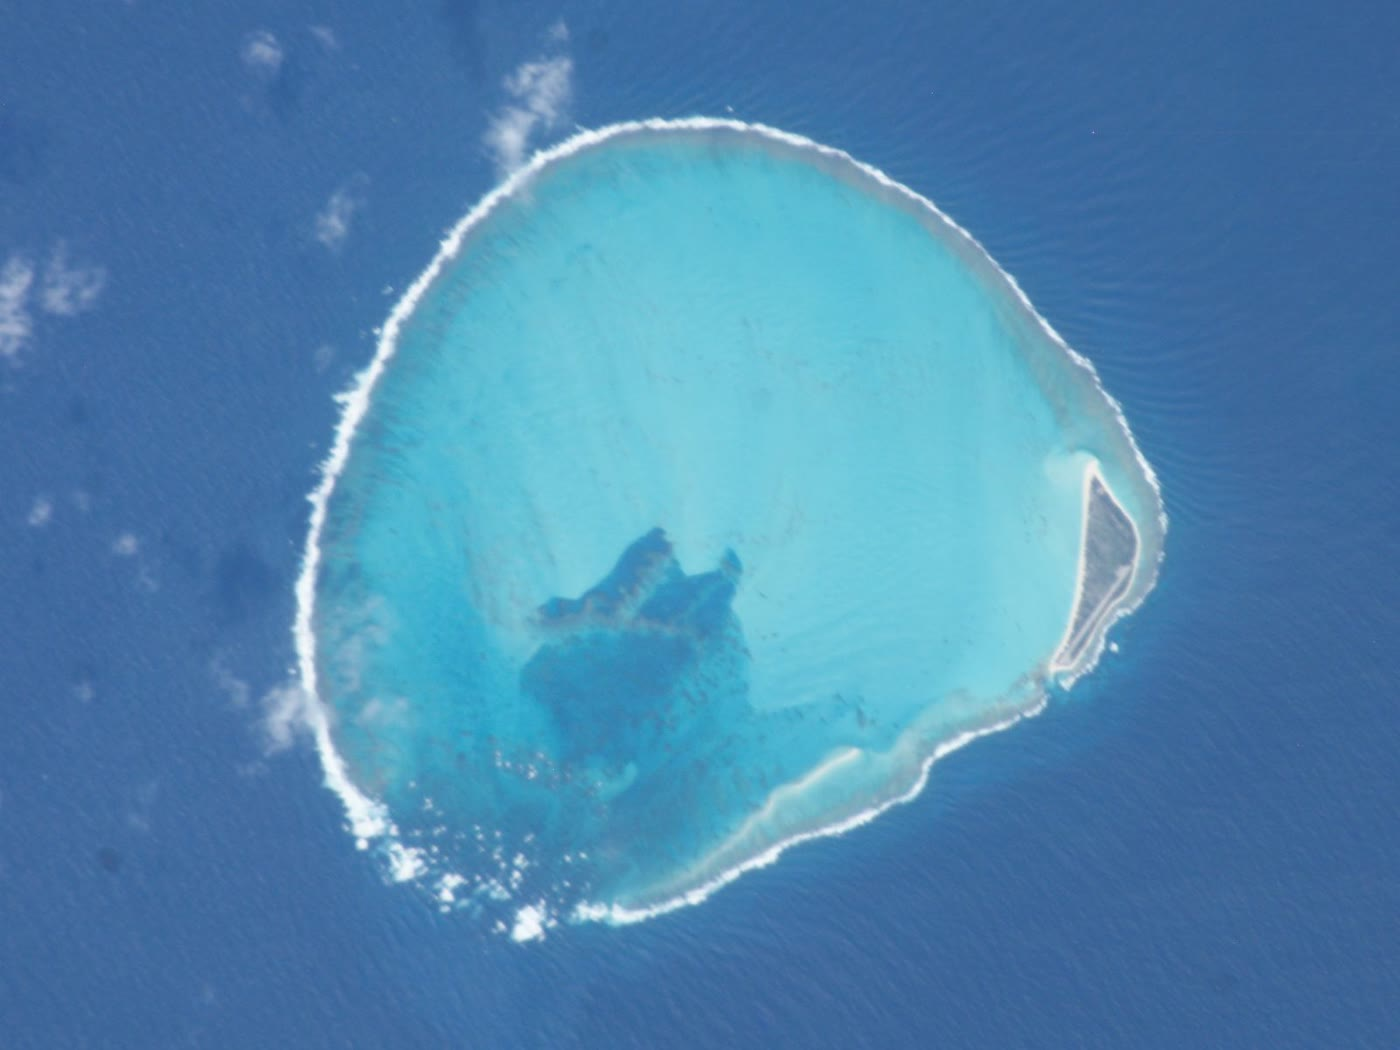
\includegraphics[width=0.52\linewidth]{images/book4/b2-17-kure-atoll.jpg}
\par\smallskip{\small Kure \omterm{def:b2:oceanic-islands:reefs}{Atoll}, the northernmost coral \omterm{def:b2:oceanic-islands:reefs}{atoll}, photographed by an astronaut from
the International Space Station on 22 February 2004. The ring of reef, about ten kilometres across
at most, encloses a lagoon; the only permanent island, Green Island, lies on the rim (right). NASA,
public domain, via Wikimedia Commons.}
\end{omfigure}
% ledger: pmnm:kure (6 miles = 9.7 km)

\section{Erosion, sea level and the end of an island}\label{sec:b2:oceanic-islands:erosion}

While it sinks, an island is also worn down. A high island catches the trade winds: on the
windward slopes of the Hawaiian volcanoes, more than \qty{9}{m} of rain falls in a year in places.
Streams cut deep canyons in less than a million years, as on Kohala, on the Island of Hawaii.
Some great cliffs once taken as the work of erosion alone, such as the sea cliffs of northern
Molokai, are now read as the headwalls of giant slides, cut back since. Waves attack the coast and
plane a wave-cut platform at sea level around it. Erosion and sinking together remove every trace
of volcanic rock above the sea in about \qty{15}{Myr}. Gardner Pinnacles, of about that age, is
the oldest island of the chain where volcanic rock still stands above the water. Beyond it to the
north-west there are only sand islands, \omterm{def:b2:oceanic-islands:reefs}{atolls} and drowned volcanoes.
% ledger: cs14:erosion, cs14:erase

Sea level does not stand still while this goes on. During the last glacial maximum it was about
\qty{120}{m} lower than today. The coast of an island then lay lower on its flanks, and the reefs
that now fringe it were dry land. When the ice melted, the sea rose by an average of \qty{12}{m}
every thousand years over the main deglaciation, from 16.5 to \qty{8.2}{ka}. During Meltwater
Pulse 1A it rose by at least \qty{40}{mm} a year. A reef on a sinking volcano must follow both
rises. Off the north-west coast of the Island of Hawaii, at least six drowned reefs form a
staircase on the flank, the oldest the deepest. Each grew at the shore, fell behind during a rise
of the sea, and was carried down by the loading of the young island. Once a volcano has sunk more
than about \qty{125}{m}, the range of glacial sea level, it will not come back up into the waves.
% ledger: usgs:lgm (Book 1), lambeck14:lgm (Book 2), cs14:erase, cs14:subsidence

The arch can work the other way. Oahu sits on the bulge raised by the load of the younger islands,
and has risen a little: reefs of the last interglacial, 133 to \qty{115}{ka} old, crop out all
round the island, and a reef about \qty{334}{ka} old now stands \qty{21}{m} above sea level. The
end of an \omterm{def:b2:oceanic-islands:stages}{oceanic island} is thus written in its rocks and its reefs. Lava builds it, slides and
rain cut it down, waves plane it, the plate carries it down, and a reef keeps its place at the
surface until cold water and a rising sea drown that too.
% ledger: cs14:arch

\section*{Exercises}\label{sec:b2:oceanic-islands:exercises}

Data for the exercises, unless stated otherwise: depth--age law $d = \qty{2500}{m} + C\sqrt t$ with
$C = \qty{350}{m.Myr^{-1/2}}$ for $0 \le t \le \qty{70}{Myr}$, and $d = \qty{6400}{m} -
\qty{3200}{m}\,e^{-t/62.8}$ beyond \qty{20}{Myr}; $1~\text{foot} = \qty{0.3048}{m}$, $1~\text{fathom}
= \qty{1.8288}{m}$, $1~\text{mile} = \qty{1.609}{km}$; reef growth up to \qty{4.2}{mm.yr^{-1}}.

\begin{exercise}[$\star$]\label{exo:b2:oceanic-islands:1}
Name the stage of each volcano: (a) a \omterm{def:b2:oceanic-islands:seamount}{seamount} whose summit is \qty{975}{m} under the sea, erupting
alkalic lava; (b) a volcano over the hotspot, erupting tholeiitic lava at a high rate; (c) an
extinct volcano whose last flows, more alkalic than the bulk of the island, cap the shield; (d) an
island where, after a silence of \qty{2}{Myr}, a few small alkalic vents open; (e) a ring of reef
around a lagoon with no volcanic rock in sight.
\end{exercise}

\begin{exercise}[$\star$]\label{exo:b2:oceanic-islands:2}
A volcano is built on a plate \qty{9}{Myr} old. (a) How deep is the sea floor around it? (b) How
far will it have sunk when the plate is \qty{25}{Myr} old? (c) At what rate is it sinking then?
\end{exercise}

\begin{exercise}[$\star$]\label{exo:b2:oceanic-islands:3}
Seventeen large slides formed in the last \qty{5}{Myr} around the main Hawaiian Islands, and
seventy along the Hawaiian Ridge in \qty{30}{Myr}. (a) Find the mean interval between two slides in
each case. (b) Why are both only upper limits of the true interval?
\end{exercise}

\begin{exercise}[$\star$]\label{exo:b2:oceanic-islands:4}
On Enewetak, basalt was met at 4,158 feet in one hole and hard basement at 4,610 feet in the
other; the reef corals at the base of the limestone do not live deeper than 150 feet. (a) Convert
the three depths to metres. (b) By at least how much has the top of the volcano under Parry Island
sunk since the first reef grew on it? (c) The base of the limestone is Eocene, so at least
\qty{33.9}{Myr} old. What is the largest possible mean rate of sinking?
\end{exercise}

\begin{exercise}[$\star\star$]\label{exo:b2:oceanic-islands:5}
(a) Find the rate of thermal sinking, in \unit{m} per \unit{Myr} and in \unit{mm.yr^{-1}}, of
islands on plates 4, 25 and \qty{49}{Myr} old. (b) How many times faster than the fastest of these
can a productive reef grow? (c) And how many times faster is the loading phase off the Island of
Hawaii, \qty{2.6}{m} per thousand years?
\end{exercise}

\begin{exercise}[$\star\star$]\label{exo:b2:oceanic-islands:6}
(a) With the exponential law, find the rate of sinking on a plate \qty{100}{Myr} old, in \unit{m}
per thousand years, and compare it with the \qty{0.01}{m} per thousand years measured along the
Hawaiian Ridge. (b) On what plate age is the rate exactly \qty{10}{m.Myr^{-1}}? (c) Check that the
two laws give nearly the same depth for a plate \qty{25}{Myr} old.
\end{exercise}

\begin{exercise}[$\star\star$]\label{exo:b2:oceanic-islands:7}
The Hawaiian reefs drown about \qty{33}{Myr} after their volcano was born, and volcanism moves
along the chain at \qty{8.6}{cm.yr^{-1}}. (a) How far from the hotspot does an island lie when its
reef drowns? (b) Midway is an \omterm{def:b2:oceanic-islands:reefs}{atoll} \qty{27.7}{Myr} old: is it consistent that it still has a
living reef? (c) Kure lies 55 miles beyond Midway. Estimate its age, and say whether it is close
to the \omterm{def:b2:oceanic-islands:darwin-point}{Darwin point}.
\end{exercise}

\begin{exercise}[$\star\star$]\label{exo:b2:oceanic-islands:8}
In the Nuuanu \omterm{def:b2:oceanic-islands:collapse}{debris avalanche}, Tuscaloosa \omterm{def:b2:oceanic-islands:seamount}{Seamount} is a block about \qty{30}{km} long,
\qty{17}{km} wide and at least \qty{2}{km} tall. (a) What volume would a box of these dimensions
hold? And a pyramid on the same base and with the same height? (b) Compare with the volume of
Kilauea, \qty{10000}{km^3}. (c) The avalanche covers \qty{23000}{km^2}. If it were on average
\qty{100}{m} thick (an assumption: its thickness far from Oahu is poorly known), what would its
volume be?
\end{exercise}

\begin{exercise}[$\star\star$]\label{exo:b2:oceanic-islands:9}
Off the Island of Hawaii the flank sinks by \qty{2.6}{m} per thousand years under the load of the
volcano. (a) How long does it take to drown a shoreline by \qty{1}{km}? (b) A reef growing at
\qty{4.2}{mm.yr^{-1}} sits on this flank. Does it keep up when sea level is steady? (c) During the
main deglaciation, from 16.5 to \qty{8.2}{ka}, the sea rose by \qty{12}{mm.yr^{-1}} on average. How
deep is the top of the reef at the end, if it started at the surface? (d) The same, for a reef on
an old volcano that no longer sinks.
\end{exercise}

\begin{exercise}[$\star\star\star$]\label{exo:b2:oceanic-islands:10}
(a) Show that, over a fixed interval $\Delta$, the root law makes an island sink less the older its
plate. (b) Compute the sinking over \qty{20}{Myr} for an island born at the ridge and for one born
on a plate \qty{50}{Myr} old. (c) The plate under a ridge is very hot, and the root law gives an
infinite rate at $t = 0$. Is that a problem for the sinking over a finite interval? Explain.
\end{exercise}

\begin{exercise}[$\star\star\star$]\label{exo:b2:oceanic-islands:11}
An \omterm{def:b2:oceanic-islands:reefs}{atoll} sinks at \qty{30}{m.Myr^{-1}}, and sea level swings by about \qty{120}{m} with the ice
ages, in cycles of about \qty{100}{kyr}. (a) How far does the \omterm{def:b2:oceanic-islands:reefs}{atoll} sink during one cycle? (b) At a
glacial lowstand, how high does the top of the \omterm{def:b2:oceanic-islands:reefs}{atoll} stand above the sea? What happens to the
reef rock then? (c) How many cycles does it take for the \omterm{def:b2:oceanic-islands:reefs}{atoll} to sink by the full \qty{120}{m}?
(d) Explain the leached zones found in the Enewetak holes, and why
\cref{prop:b2:oceanic-islands:cap} still gives the thickness of the cap over the long run.
\end{exercise}

\begin{exercise}[$\star\star\star$]\label{exo:b2:oceanic-islands:12}
An \omterm{def:b2:oceanic-islands:reefs}{atoll} drowns when its plate is \qty{50}{Myr} old: its reef falls behind and its top ends at the
growth limit of the deepest coralline algae, \qty{150}{m} under the sea. (a) With the exponential
law, how much further does it sink before the plate is \qty{120}{Myr} old? (b) How deep is the top
of the \omterm{def:b2:oceanic-islands:seamount}{guyot} then? (c) A \omterm{def:b2:oceanic-islands:seamount}{guyot} beside Enewetak has its top at 700 fathoms. Convert, and compare.
(d) Name two reasons why a real \omterm{def:b2:oceanic-islands:seamount}{guyot} could be deeper or shallower than this estimate.
\end{exercise}

\begin{problem}[{Weekend problem --- From volcano to atoll}]\label{pb:b2:oceanic-islands:1}
The invented Petrel Island is born over a hotspot on a plate \qty{10}{Myr} old. Its volcano is
a cone of basal radius \qty{50}{km}. When its growth ends, its summit stands \qty{1000}{m} above
sea level. Its last volcanic rock disappears below sea level \qty{12}{Myr} later. A reef then
keeps its top at sea level until the plate is \qty{70}{Myr} old, when the \omterm{def:b2:oceanic-islands:reefs}{atoll} crosses the
\omterm{def:b2:oceanic-islands:darwin-point}{Darwin point}. Use the depth--age law of the exercises (the root law up to \qty{70}{Myr}, the
exponential law beyond), a reef growth of \qty{4.2}{mm.yr^{-1}}, and the data of the chapter.
Sea level is taken as constant, except in questions 8 to 10. Round depths to the metre.

\noindent\textbf{Part I --- Growth.}
\begin{enumerate}
  \item How deep is the sea floor where Petrel is born?
  \item What is the height of the volcano above that floor when its growth ends, ignoring the
        sinking of the floor under the load?
  \item Find the volume of the cone.
  \item If \qty{85}{\percent} of it erupted during a \omterm{def:b2:oceanic-islands:stages}{shield stage} of \qty{1}{Myr}, what was the
        mean rate of eruption? Compare with the supply of Kilauea today, about
        \qty{0.1}{km^3} a year.
  \item How many Petrels would make one Mauna Loa, at \qty{95600}{km^3}?
  \item Which lavas, tholeiitic or alkalic, make up most of the cone? Which cap it?
\end{enumerate}

\noindent\textbf{Part II --- Loading and drowned reefs.}
\begin{enumerate}[resume]
  \item During its growth, the load sinks the young island by \qty{1}{km} in \qty{1}{Myr}. What is
        the mean rate, and how does it compare with the \qty{2.6}{m} per thousand years measured
        off the Island of Hawaii?
  \item A reef grows on the shore during this phase, with sea level steady. Does it keep up, and
        with what margin?
  \item Sea level then rises by \qty{12}{mm.yr^{-1}}. By how much does the reef fall behind each
        year?
  \item How long before its top reaches \qty{150}{m}, the deepest growth limit? What does that
        leave on the flank of the island?
\end{enumerate}

\noindent\textbf{Part III --- Sinking and erosion.}
\begin{enumerate}[resume]
  \item By how much has Petrel sunk by the time its last volcanic rock disappears, the plate being
        then \qty{22}{Myr} old?
  \item How much of the \qty{1000}{m} of the summit did erosion remove, and at what mean rate?
  \item At what rate is Petrel sinking when its growth ends, and when its summit disappears?
  \item How deep is the sea floor around it then?
  \item Compare the \qty{12}{Myr} it took with the \qty{15}{Myr} of the Hawaiian Islands. Give a
        reason why a high Hawaiian island lasts longer.
  \item Name two processes, besides rain and rivers, that remove the island above sea level.
  \item Which form of reef surrounds Petrel shortly before its summit disappears?
\end{enumerate}

\noindent\textbf{Part IV --- Atoll and guyot.}
\begin{enumerate}[resume]
  \item How thick is the reef cap when the plate is \qty{70}{Myr} old?
  \item What mean rate of reef growth did that need? How many times smaller is it than the growth
        the reef could reach?
  \item Compare the cap with the depth of the basalt under Enewetak.
  \item How deep is the sea floor around the \omterm{def:b2:oceanic-islands:reefs}{atoll} when it crosses the \omterm{def:b2:oceanic-islands:darwin-point}{Darwin point}?
  \item With the exponential law, how much further does the drowned \omterm{def:b2:oceanic-islands:reefs}{atoll} sink before the plate is
        \qty{120}{Myr} old?
  \item If the top of the reef stopped at \qty{150}{m} when it drowned, how deep is the top of the
        \omterm{def:b2:oceanic-islands:seamount}{guyot} then?
  \item To sum up: how thick is the reef cap of Petrel \omterm{def:b2:oceanic-islands:reefs}{atoll}?
\end{enumerate}
\end{problem}
